\documentclass[british]{article}
\usepackage[utf8]{inputenc}
\usepackage[british]{babel}% Recommended
\usepackage{csquotes}% Recommended

\usepackage[sorting=nyt,style=apa]{biblatex}

\addbibresource{~/Tex/library.bib}
\usepackage[toc,page]{appendix}
\usepackage[margin=1in]{geometry}

\usepackage{amsmath}
\usepackage{graphicx}
\usepackage{listings}
\usepackage{enumerate}
\usepackage{booktabs}
\usepackage{wrapfig}
\newcommand{\code}[1]{\texttt{#1}}
\newtheorem{defin}{Definition}
\newtheorem{prop}{Proposition}
\newtheorem{col}{Corollary}
\newtheorem{thm}{Theorem}
\setlength{\parskip}{1em}
\usepackage{placeins}

%Default fixed font does not support bold face
\DeclareFixedFont{\ttb}{T1}{txtt}{bx}{n}{12} % for bold
\DeclareFixedFont{\ttm}{T1}{txtt}{m}{n}{12}  % for normal

% Custom colors
\usepackage{color}
\definecolor{deepblue}{rgb}{0,0,0.5}
\definecolor{deepred}{rgb}{0.6,0,0}
\definecolor{deepgreen}{rgb}{0,0.5,0}

\usepackage{listings}

% Python style for highlighting
\newcommand\pythonstyle{\lstset{
		language=Python,
		breaklines=true,
		frame=single,
		numbers=left,
		tabsize=2,
		basicstyle=\ttm,
		otherkeywords={self},             % Add keywords here
		keywordstyle=\ttb\color{deepblue},
		emph={MyClass,__init__},          % Custom highlighting
		emphstyle=\ttb\color{deepred},    % Custom highlighting style
		stringstyle=\color{deepgreen},
		frame=tb,                         % Any extra options here
		showstringspaces=false            % 
}}


% Python environment
\lstnewenvironment{python}[1][]
{
	\pythonstyle
	\lstset{#1}
}
{}

% Python for external files
\newcommand\pythonexternal[2][]{{
		\pythonstyle
		\lstinputlisting[#1]{#2}}}

% Python for inline
\newcommand\pythoninline[1]{{\pythonstyle\lstinline!#1!}}

\title{CS4402 - Practical 1: Bombastic}
\author{170008773}
\date{\today}

\begin{document}
	\maketitle
	
	
	\begin{abstract}
		The planning of sequences of moves is a common problem in constraint solving,  applicable in problems like scheduling to route planning. To be able to solve these problems efficiently they have to be modelled in such a way that solvers can work with the data efficiently. Here it is critical to note that the way these problems are modelled can have potentially huge impacts on how efficiently they can be solved. As an exercise in constraint modelling, I have modelled the game Bombastic in Essense Prime. In this report, I will detail the design choices, the testing of the model and the results of benchmarking the model with different levels of optimisation performed by the solver. I found that for the smaller problems there is not that much difference between the levels of optimisation but as the problems become more complex both using no optimisation and all the possible optimisation have significantly worse performance than using a moderate amount of optimisation.  	
	\end{abstract}
	
	\section{Problem description}
	I will first start with a description of the problem I modelled. 
	\label{problem}
	\subsection{The game}
	Bombastic is played on an $N\times M$ grid of cells. The cells in this grid can either be \code{dead}, \code{ice}, or \code{normal}. \code{dead} cells can be entered by neither the blocks nor the avatar, and other cells can accommodate at most one block or the avatar. For simplicity's sake, we assume that every grid is surrounded by a wall of dead cells. On this grid, there is an avatar and one or more blocks and a number of goals, \textit{equal to the number of blocks}. The objective of the avatar is to walk around the grid and push the blocks around until all blocks are at a goal. In this scenario, we are not interested in which block ends up at which goals.  
	
	
	\subsection{Avatar logic}
	The avatar is allowed to move around the grid, moving the cell it is currently occupying to any of the adjacent empty cells that are not dead. The avatar is only allowed to move purely horizontally or vertically (i.e. not at the same time) and not moving is also disallowed.  The player is allowed to move onto an ice cell but when it moves off that cell again, the ice will crack, turning the cell into a dead one. 
	
	
	\subsection{Box logic}
	The avatar can move blocks by moving into their square. This will move the block one square in the direction in which the avatar is travelling. This is only allowed if the cell into which the block is moving is not dead and does not contain another block. The avatar may only allowed to push one block at a time.
	
	\subsection{Objectives}
	Given the grid layout, the positions of the blocks, the position of the goals, and the initial position of the avatar, the objective is to find a sequence of legal avatar moves that move all the blocks such that every goal is occupied by a block. In this instance, the number of moves is provided. The problem is then to find whether there is a sequence of the given length that satisfies all the objectives and constraints. 
	
	
	\section{Modelling the problem}
	I will now detail how the assignment was set up, the major modelling ethos used and the new instances I designed. 
	\label{model}
	\subsection{Setup}
	In this instance, I was required to use the modelling language \code{Essence prime} in conjunction with the constraint solver Savile Row. I was also provided with the decision variables, their domains and several sets of parameters to test the system. I was required to add the constraints to accurately model the problem and solve the provided instances, as well as design several new instances. 
	
	\subsection{Modelling decisions}
	\paragraph{Redundancy}
	As mentioned previously, the way the problems are modelled can have big impacts on how efficiently they are solved. The fewer constraints there are to check, the less work the solver has to perform. So there is an incentive to make the constraints as simple and as small in number as possible. On the other hand, however, these models, even ones that are well constructed, can be very complex to interact with on a human level. To mitigate this, extra constraints that overlap with, or even imply other constraints can be used as sanity checks. Ultimately, these are judgement calls as either extreme is likely to cause problems. In the modelling of this problem, I opted to lean towards redundant constraints, feeling that an extreme focus on performance was not needed considering the scope of the project. 
	
	Note however that this can significantly increase the work in heavily optimised runs, especially if the constraints are simple, checking them might not be a problem. However, it might be less simple to reduce them to common expressions etc. which is what the highest level of optimisation tries to do. Later in section \ref{results} we will see that in the more complex instances, the heavily optimised runs can struggle hugely. This is one of the possible causes of that. 
	
	\paragraph{Elegance} In contrast to redundancy, it benefits both human and machine to simplify the constraints as much as possible. This practice can make the model more understandable to humans and easier to solve for the machine. Where possible I attempted to make the constraints as small as possible, trying to eliminate conjunctions or disjunctions where possible. 
	
	\paragraph{Global constrains} It is also worth mentioning that I tried to use global constraints such as \code{GCC} where possible. This was done because constrains solvers can often handle global constraints more efficiently than individual constraints. This, however, was not always possible. I chose readability over the use of global constraints since I did not think that the potential performance increases of using complicated global constraints would be worth the decrease in readability.
	
	\subsection{Model description}
	\paragraph{Overview} The model is roughly divided into four parts: Initialisation, Game logic, Avatar logic and Box logic, each of which I will discuss below. 
	
	\paragraph{Initialisation} This is fairly straightforward. I was given the initial positions for the goals, the blocks, the map layout and the avatar. In this section, I simply looped over all our environment variables at time 0 and set them to the initial parameters received. 
	
	\paragraph{Game logic} The game logic section is mainly concerned with detailing the end conditions of the game, namely that all the goals must be occupied by a block, and how the cells in the map are or are not supposed to change. Here I chose to add some redundant constraints  as a sanity check, which state that normal cells stay normal and dead cells stay dead. Finally, ice cells crack when the avatar leaves them. Since not moving is disallowed, we did this by checking when the avatar enters the ice cell and killing the cell in the next step.
	
	\paragraph{Avatar logic} The avatar logic is also relatively straightforward. Avatars cannot enter dead cells, their position should be updated using the \code{moveCol} and \code{moveRow} variables and they are only allowed to move one square in either a vertical or horizontal direction. I chose to model the movement using the sum of the absolute values of the move variables because this simultaneously details which moves are allowed and disallow both diagonal movement and non-movement. 
	
	\paragraph{Box logic} Box movement is the most complicated part of this model since it involves the greatest number of variables. Making a block move involves checking the blocks' position, the position of the avatar, the direction in which the avatar wants to move and the position to which the block itself would move. Here it is useful to note that we must add constraints that blocks are not allowed to move unless pushed by the player, to avoid the solver simply teleporting them to the goals at any point in time. Because this is the most complex part of the model we have opted to leave in the most redundant constraints. For example, the constraint that blocks can share a cell would have been sufficient to ensure that no two blocks can be pushed simultaneously, but since this depends on how the movement of the avatar is checked, we decided to add a separate constraint for this as a sanity check. 
	
	
	\subsection{Designed instances}
	I was also required to design new instances of this problem class. I took this opportunity to design a few instances that can be used to either test specific parts of the modelled logic or some artificially difficult problem to test the performance. They are designed in pairs. Every problem has one parameter file that is solvable and one that isn't so that we can see how the performance compares to comparable problems. To make the process of visualising the results a little easier every impossible version of an instance requests a solution that is 1 step shorter than the shortest solution, even if it is made impossible by other modifications. We will discuss them below. Humanly readable maps of all the instances are provided in the files. The numbers in the list correspond to the appropriate file name. 
	\begin{enumerate}[1)]
		\setcounter{enumi}{9}
		\item This problem is a slight adaptation of the \code{Bombastic1\_1.param}. It is a single-width corridor with two blocks in it. This is designed to test the avatar's inability to push more than one block at the same time.
		\item This is another instance designed to test the ice mechanic. There is an L shaped corridor with an ice cell at the intersection on which the avatar starts and a block and goal in each branch. The possible version removes the ice cell. 
		\item This problem contains a square of ice in the middle with two single-width corridors with a block on either end. The possible version has one ice cell replaced with a normal one, making it possible. This instance was designed to test how the solver deals with ice planning, and whether the ice mechanic is done correctly. 
		\item This instance is a slightly more complicated instance to test the inability of the avatar to push more than one box at a time. It has a small room and two blocks in a row with goals on two sides. This instance requires a tiny bit of planning since the avatar will First have to walk around the blocks.
		\item This instance is simply a large open room with no complications. It is designed to test how the solver performs in terms of the length of the solutions and the size of the possible moves while the actual solution is very uncomplicated.
		\item  This instance is a simple adaptation of \code{Bombastic9\_17.param}.  It is identical to the old instance but it has a relatively big empty space added at the bottom that should change nothing about the solution. This was done to test how well the solver would fare if a lot of useless space was added.
	\end{enumerate}
	
	\section{Emperical evaluation}
	\label{results}
	In this section, I will describe the testing process used and discuss the results. Savile Row has several levels of optimisation (levels 0 through 3). In these levels, it performs different optimisation steps. These steps include but are not limited to common subexpression elimination, unifying equal variables and filtering domains. These optimisations can save work during the search phase but can also be quite expensive themselves, making them potentially useless or even worse. Here we perform empirical analyses to see how the different levels of optimisation compare.  
	
	\subsection{Testing process}
	\label{testing}
	The testing process was fairly straightforward. In addition to the testing I did while designing the system, I used both the provided instances as well as my own designed instances described above. As discussed above I designed some instances with the intention of testing specific aspects of the model and others were designed to test the overall performance of the model. 
	
	I used a python script to run the solver on every instance with all the optimisation levels and automatically record the data. This data consisted of an instance id, the number of steps of the requested solution, the optimisation level, whether a solution was found and the computation time taken by the solver. I measured the computation time in CPU seconds spent in user mode (as described by the bash module \code{time}).  The remaining data was obtained by a simple parsing of the output, the solver and parameter file. The code for the script can be found in appendix \ref{collection}. The script should be run as \code{`python timer.py`} and it will recursively search through the directory tree from where it was called and process all the \code{.param} files it finds. 
	
	\subsection{Results}
	In this section, I will discuss the computation time of Savile Row as a function of two measures: the level of optimisation and the length of the requested solution. As can be seen in table \ref{compstats} the computation time varies very little for levels 1 and 2, but can vary an enormous amount for levels 0 and 3 as will be discuss in more detail below 
	%\begin{wrapfigure}{l}{0.4\textwidth}]
	\begin{figure}[!h]
		\centering
		\begin{tabular}{lrr}
			\toprule
			{} & \multicolumn{2}{l}{compTime} \\
			{} &        mean &         std \\
			optLevel &             &             \\
			\midrule
			0        &  327.668276 &  931.351282 \\
			1        &    6.343345 &    4.575549 \\
			2        &    7.345448 &    4.839894 \\
			3        &  213.884966 &  679.810891 \\
			\bottomrule
		\end{tabular}
		\caption{Computation time statistics by level of optimisation}
		\label{compstats}	
		
	\end{figure}
	%\vspace{-55pt}
	%\end{wrapfigure}
	
	\subsubsection{Computation per step}
	Because of the intricate nature of constraint problems, in general, I cannot make precise claims about space or time complexity of these problems. Therefore I will only discuss the empirical results found. In figure \ref{stepsVsCPUSec} you will find the computation times of all the instances that failed.
	\FloatBarrier
	\begin{figure}[!ht]
		\centering
		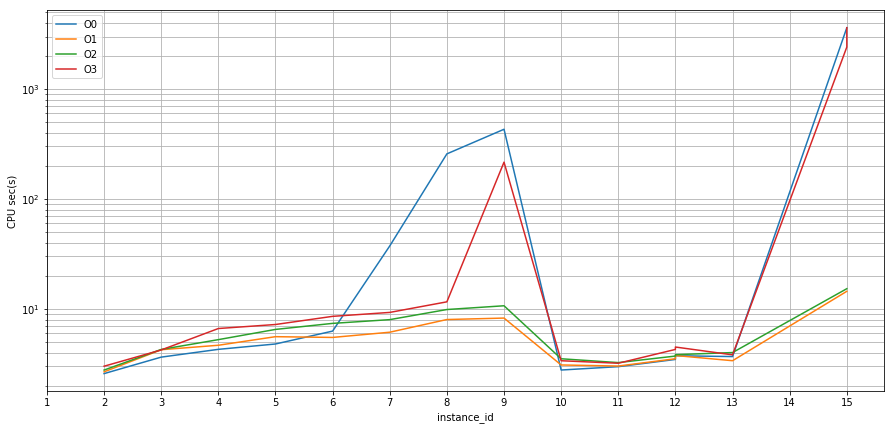
\includegraphics[width=0.9\textwidth]{idVsCPUSec}
		\caption{The instance id vs. user CPU time. (lower is better) User IDs of the designed instances are arranged to have increasing step sizes.}
		\label{idVsCPUSec}	
	\end{figure}
	\FloatBarrier 
	
	When the problems are relatively small, the level of optimisation doesn't matter that much. For the simpler problems, the least number of optimisation seems to be best, which makes sense since the extra overhead of optimisation might not be worth it for such small problems. As we increase the length of the requested solution we see that levels 1 and 2 remain roughly linear. Optimisation level 0 and 3 however, eventually start exhibiting exponential behaviour. For level 0 this is what we expected since the search space grows too fast if we don't make smart optimisations for this. The dip that happens around 10 is because that is the threshold for the designed instances which start out with a low step length.
	
	\paragraph{Heavy optimisation} What happens to level 3, however, is slightly more counter-intuitive. This can explained as follows: Optimisation is a lot of work and if the search space is less conducive to optimisation it can waste a lot of effort. I assume that this is what happened since I was not able to model the problem using many global constraints. These global constraints are easiest the optimise away, so the fact that we didn't use them that much might make the heavy optimisation not worthwhile. As we mentioned earlier this is where the solver can spend a lot of extra time trying to optimise our redundant constraints away. 
	
	\subsubsection{Complexity vs length} 
	
	When looking at the tail end of the graph above, it is clear that while levels 1 and 2 perform fairly well with longer solutions, levels 0 and 3 start performing quite badly. Now I will examine the difference between level 0 and level 3 more closely. 
	
	Here it is useful to look at the instances I designed (number 14 and 15 specifically). These contain large open spaces that do not serve any special purpose. Here we can see that Level 3 solidly outperforms level 0. Presumably, because it doesn't get stuck walking around in the large spaces, offsetting the cost of the optimisation. I presume that this trend would continue as the length of the requested solutions continues to grow. 
	
	\paragraph{Relative performance of instances} In this context it is also useful to compare the performances of the same instance between the possible and impossible versions since these have similar (or identical) complexity but differing solution lengths. The relative difference between the computation times of the same instance can be found in figure \ref{idVsCPUSecDiffed} below.  
	\begin{figure}[!ht]
		\centering
		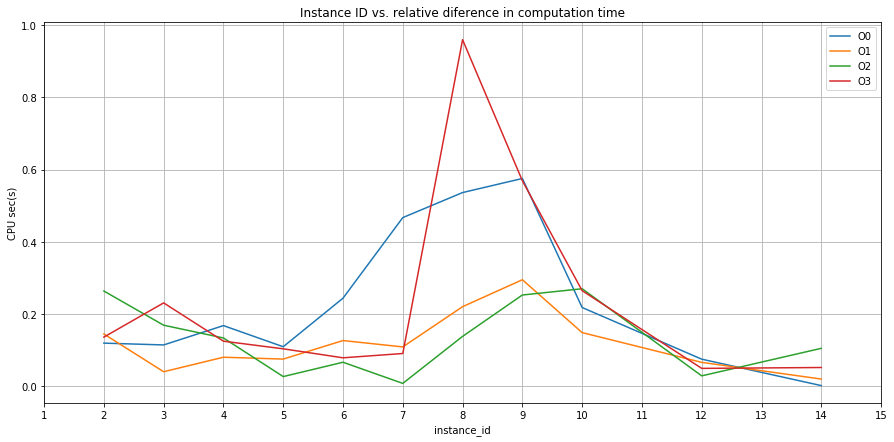
\includegraphics[width=0.9\textwidth]{idVsCPUSecDiffed}
		
		\caption{The instance id vs. absolute difference of user CPU time between the possible and impossible variant of every instance. User IDs of the designed instances are arranged to have increasing step sizes.}
		\label{idVsCPUSecDiffed}
	\end{figure}
	\FloatBarrier
	
	Looking at the graph, we see that the relative difference in computing time roughly increases with the \code{instance\_id} i.e. with higher solution length.  This also makes sense since at higher steps adding another step increases the possible state space to search, but much more than adding steps to small spaces. It is clear that again level 0 and level 3 have the highest difference, with 3 having the highest of all. This makes sense since level 0 must traverse almost all of the search space, a single step increase can have big consequences. Conversely, heavily optimised runs could possibly find solutions much faster when a solution is possible creating a big difference to when there is no solution and it has to search an entire space anyway, effectively wasting the optimisation time. 
	
	\section{Conclusion}
	\label{conclusion}
	For this assignment, I modelled an abstracted version of the game Bombastic. In this report, I discussed the rules and how I modelled them using Savile Row. Eventually,I found that both optimisation levels 0 and 3 produced less than optimal results, with level 2 performing best across the board. 	
	
	
	word count: 2732
	
	\FloatBarrier
	\begin{appendices} 	
		\section{Data collection script}
		\label{collection}
		\pythonexternal{../timer.py}
	\end{appendices}
	
	
	\printbibliography
\end{document}